% Manual, as well as usage example, for the titlepic.sty package.
% Run this through latex to see the output.

\documentclass[titlepage]{article}

\usepackage[cc]{titlepic} % Include the titlepic package.

% Creates a placeholder for the picture (no real picture is included in the package to keep it small).
% The syntax is \placeholder{width}{height}.
\newcommand\placeholder[2]{%
	\noindent%
	{\setlength{\fboxsep}{0pt}%
		\framebox[#1]{%
			\parbox{0pt}{\rule{0pt}{#2}}%
			\parbox{#1}{\centering The picture goes here.}%
		}%
	}%
}

\title{\LaTeX{} \texttt{titlepic} Manual}
\author{
	Thomas ten Cate\thanks{\texttt{<ttencate@gmail.com>}} \\
	with contributions from \\
	Denis Bitouz\'e}
\date{March 14, 2017}
\titlepic{\placeholder{\textwidth}{0.75\textwidth}} % This is the magic command!

\begin{document}

\maketitle

\section{Introduction}

In \LaTeX, there is by default no way to put a picture on the title page or cover page that is produced by \verb$\maketitle$. Surprisingly, no package seemed to exist for this either, which is why I put together this very simple package named \verb$titlepic$.

\textbf{Note:} \verb$titlepic$ only works with the default document classes \verb$article$, \verb$report$ and \verb$book$. However, it works both with the \verb$titlepage$ and \verb$notitlepage$ document class options.

\section{Installation}

There are several ways to install the package:
\begin{itemize}
	\item Simply drop \verb$titlepic.sty$ in the same directory as your \verb$.tex$ source document. This is the easiest option for casual use.
	\item Put \verb$titlepic.sty$ somewhere in your \verb$texmf$ tree and rehash. The details depend on your \TeX{} distribution. This gives you a system-wide installation.
	\item Install it from \TeX{} Live or MiK\TeX.
\end{itemize}

\section{Usage}

Include the package as normal, with:

\begin{quote}
	\verb$\usepackage{titlepic}$
\end{quote}

\noindent If you want to be able to include a picture, then you also need

\begin{quote}
	\verb$\usepackage{graphicx}$
\end{quote}

Then, along with the usual \verb$\title$, \verb$\author$ and \verb$\date$, put a command like the following:

\begin{quote}
	\verb$\titlepic{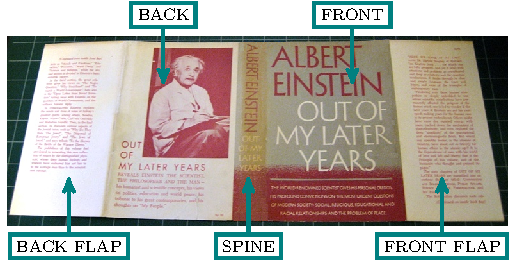
\includegraphics[width=\textwidth]{cover.png}}$
\end{quote}

The argument to \verb$\titlepic$ will usually be an \verb$\includegraphics$ command, which produces a picture. You can change the size using the optional argument to \verb$\includegraphics$, for example, \verb$width=0.7\textwidth$. This will make the picture be 70\% as wide as the text, and scales the height accordingly.

In fact, the argument to \verb$\titlepic$ can actually be pretty much anything. The output produced by this argument will be typeset centred on the title page when you invoke \verb$\maketitle$.

\section{Package options}

There are three optional arguments that control the vertical layout of the title page:

\begin{description}
\item[\tt{tt}]
	Put both the title (and author, and date) and the picture at the top of the page, separated by a fixed amount of space.
\item[\tt{tc}]
	Put the title at the top of the page as with tt, but centre the picture vertically on the page.
\item[\tt{cc}]
	Separate the title and the picture by a fixed amount of space, and centre both together vertically on the page.
\end{description}

\section{Example}

Here is a full example of what your document could look like.

\begin{verbatim}
% Pass titlepage to the article class
\documentclass[titlepage]{article}

% Centre the picture and the title vertically with cc (only works with titlepage mode)
\usepackage[cc]{titlepic}

% For \includegraphics
\usepackage{graphicx}

\title{Example}
\author{John Doe}
\date{\today}

% Now, put a picture on the title page!
\titlepic{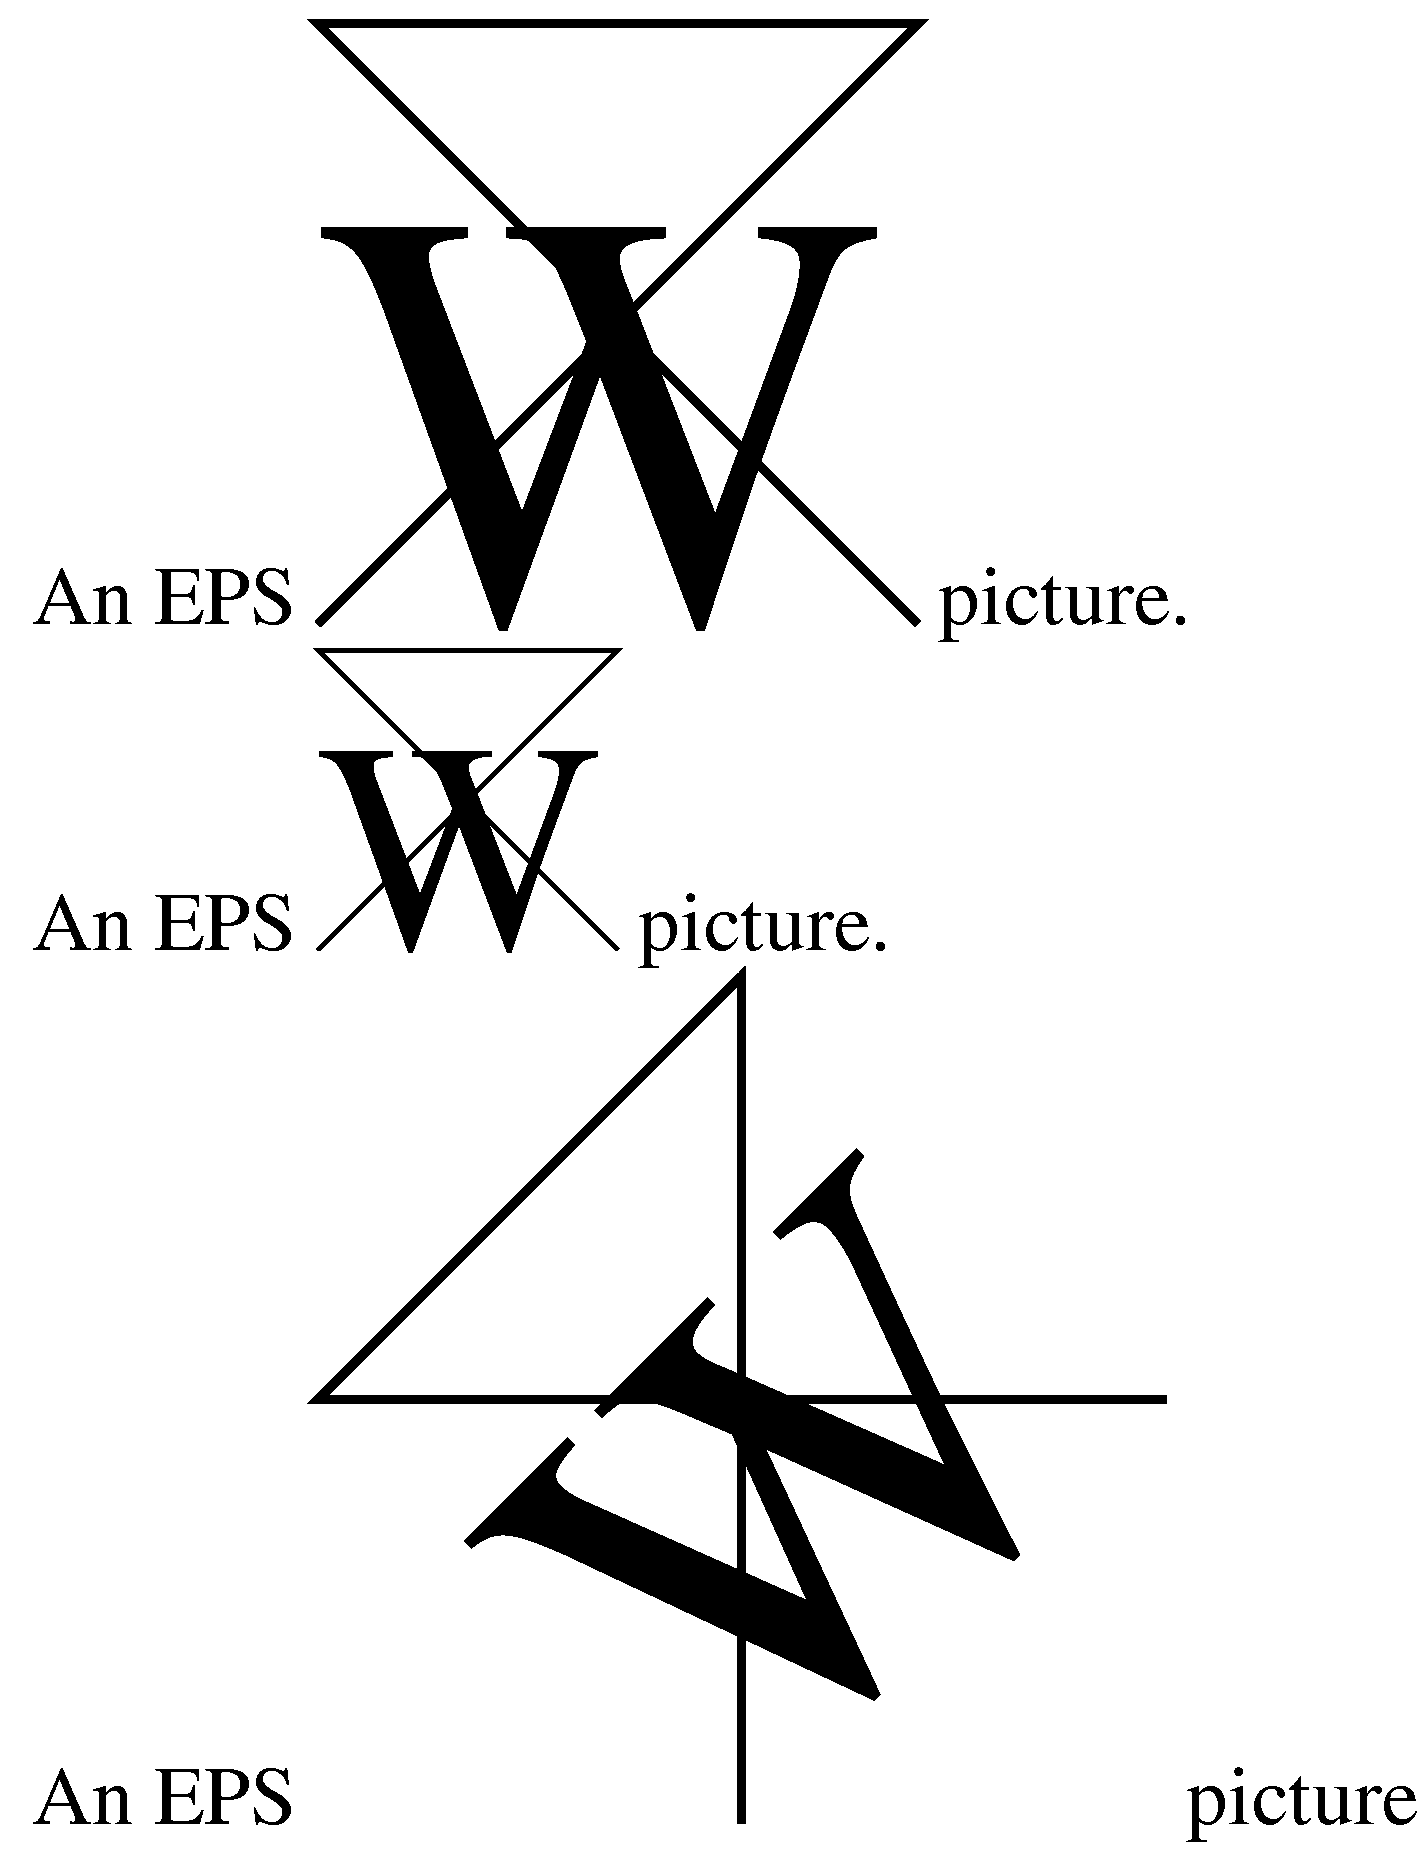
\includegraphics[width=\textwidth]{picture.png}}

\begin{document}

\maketitle

...

\end{document}
\end{verbatim}

\section{Contributing}

Contributions are welcome! Send a pull request on GitHub here:\\
\verb$https://github.com/ttencate/titlepic$

\end{document}
